\documentclass{article}
\usepackage{tikz}
\begin{document}

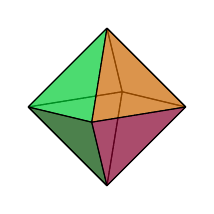
\begin{tikzpicture}[line join=bevel,z=-5.5]
\coordinate (A1) at (0,0,-1);
\coordinate (A2) at (-1,0,0);
\coordinate (A3) at (0,0,1);
\coordinate (A4) at (1,0,0);
\coordinate (B1) at (0,1,0);
\coordinate (C1) at (0,-1,0);

\draw (A1) -- (A2) -- (B1) -- cycle;
\draw (A4) -- (A1) -- (B1) -- cycle;
\draw (A1) -- (A2) -- (C1) -- cycle;
\draw (A4) -- (A1) -- (C1) -- cycle;
\draw [fill opacity=0.7,fill=green!80!blue] (A2) -- (A3) -- (B1) -- cycle;
\draw [fill opacity=0.7,fill=orange!80!black] (A3) -- (A4) -- (B1) -- cycle;
\draw [fill opacity=0.7,fill=green!30!black] (A2) -- (A3) -- (C1) -- cycle;
\draw [fill opacity=0.7,fill=purple!70!black] (A3) -- (A4) -- (C1) -- cycle;
\end{tikzpicture}

\end{document}